\section{Cubic Subspace Instance Construction}
\frame{\tableofcontents[currentsection]}


\begin{frame}
    \frametitle{Plane and Point Generation}
    \begin{figure}[ht]
        \begin{minipage}{0.5\textwidth}
            \textbf{Plane Generation:}
            \begin{itemize}
                \onslide<1->{
                \item generate 3 planes\\
                as distinct normal vectors $\vec{n}_1, \vec{n}_2, \vec{n}_3$ (normalized)
                }
                \onslide<2->{
                \item compute a $\vec{r}_{i,1}$ (normalized) orthogonal to $\vec{n}_i$
                ($i \in \{1,2,3\}$)
                }
                \onslide<3->{
                \item compute the $\vec{r}_{i,2}$ (normalized) orthogonal to $\vec{n}_i$ and $\vec{r}_{i,1}$
                }
            \end{itemize}
        \end{minipage}
        \begin{minipage}{0.48\textwidth}
            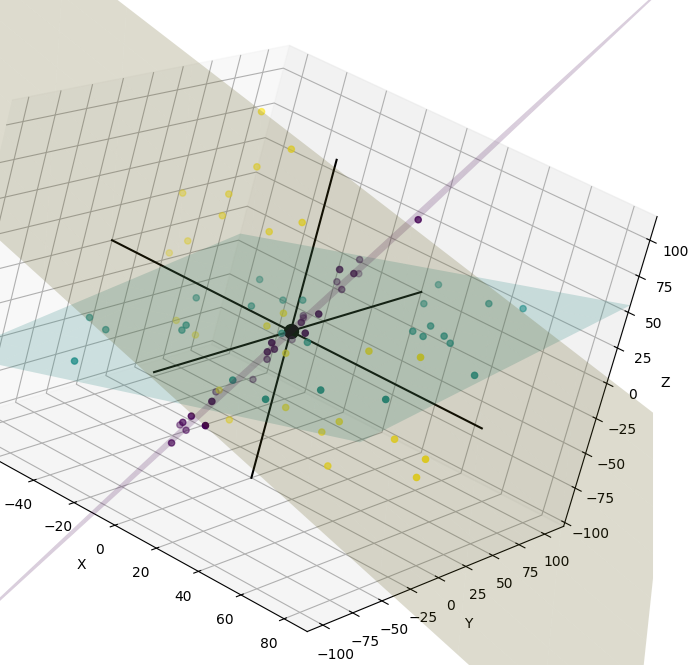
\includegraphics[width=\textwidth]{generated-points.png}
        \end{minipage}
    \end{figure}
    \onslide<4->{
    \textbf{Point Generation} on the plane $(\vec{n},\vec{r}_1,\vec{r}_2)$, parameters $(\maxD,\noise)$:
    \begin{itemize}
        \item random variables $k_1,k_2 \in [-\maxD,\maxD]$ (uniform distribution)
        \item random variable $k_n$ (normal distribution based on $\noise$) 
        \item generate point $p = k_1\vec{r_1} + k_2\vec{r_2} + k_n\vec{n}$ 
    \end{itemize}
    }
\end{frame}


\begin{frame}
    \frametitle{Cost Function}
    % cost function explain what works, what not and why do we need this conditions
    % cost function ~7min with pictures, explain ideas
    % My contribution!!! 
    % Cost function does not depend on the point distribution bounds!!!
    % Steps to assign the cost !!!!!
    % 1. skip triangle where 2 points are close to each other
    % 2. skip line like triangles
    % 3. assign penalty if the noise sum is too large
    Triangle $abc \in \binom{\fSet}{3}$
    \begin{enumerate}
        \item Smallest side $s < \maxD/2$
        $\to \cost_{abc} = 0$
        \item Largest angle $\alpha > 150\degree$
        $\to \cost_{abc} = 0$
        \item $ha,hb,hc$: distances to the best fitting plane\\
        $ha + hb + hc > 3\noise + \tol$\\
        $\to \cost_{abc} = \frac{(ha + hb + hc) - (3\noise + \tol)}{3\maxD}$
        \item $ho$: distance from the origin to the triangle plane\\
        $ho > \frac{10\noise}{\#points} + \tol$
        $\to \cost_{abc} = 0$
        \item for all points $p$:
        $hp$: distance to the best fitting plane\\
        choose $p$ if $hp < \noise + \tol$ and $|\vec{p}| > 0.3\maxD$\\
        $hp'$: distance to the best fitting plane of all chosen points\\ 
        $\delta_p = \frac{hp' - (\noise + \tol)}{\maxD}$,
        $SAME = \{p \colon \delta_p < 0\}$,
        $rew = \sum\limits_{p \in SAME} \delta_p$,\\
        $|SAME| \leq 3 \to \cost_{abc} = 0$\\
        else $\to \cost_{abc} = 2^{|SAME|-4}rew$
    \end{enumerate}
\end{frame}
